\section{Définition des axes thématiques}
\label{sec:2_axes_definition}

\subsection{Genèse et justification de la structuration thématique}

Ce découpage en sept axes n'est pas arbitraire : il résulte d'une démarche inductive, construite par analyse croisée des documents institutionnels de référence et affinée par itérations successives. Le point de départ a été l'examen approfondi de cinq sources fondatrices : le rapport Pascal-Taddei remis au MESR en juillet 2025, le référentiel UNESCO de compétences en IA pour les enseignants, la note INRIA sur l'IA générative, le cadre d'usage du MEN et la charte INSP~\cite{pascal2025ia,unesco2024competences,inria2025note,men2025cadre,insp2025charte}. Cette analyse initiale a révélé une convergence remarquable autour de quatre principes directeurs — responsabilité humaine, transparence, protection des données, formation — mais aussi des lacunes conceptuelles pour une école d'ingénieurs, particulièrement sur les projets industriels confidentiels, l'apprentissage du code et la gestion des données de recherche partenariale.

Le cadre d'analyse retenu s'organise selon trois cercles concentriques, du général au particulier : le niveau \textit{macro} (cadres internationaux et nationaux), le niveau \textit{méso} (enseignement supérieur et écoles d'ingénieurs) et le niveau \textit{micro} (Polytech Annecy-Chambéry et l'USMB). Cette architecture, inspirée des approches écosystémiques en sciences de l'éducation, permet d'articuler les contraintes réglementaires descendantes avec les réalités de terrain ascendantes (Figure~\ref{fig:cercles_concentriques}).

\begin{figure}[htbp]
\centering
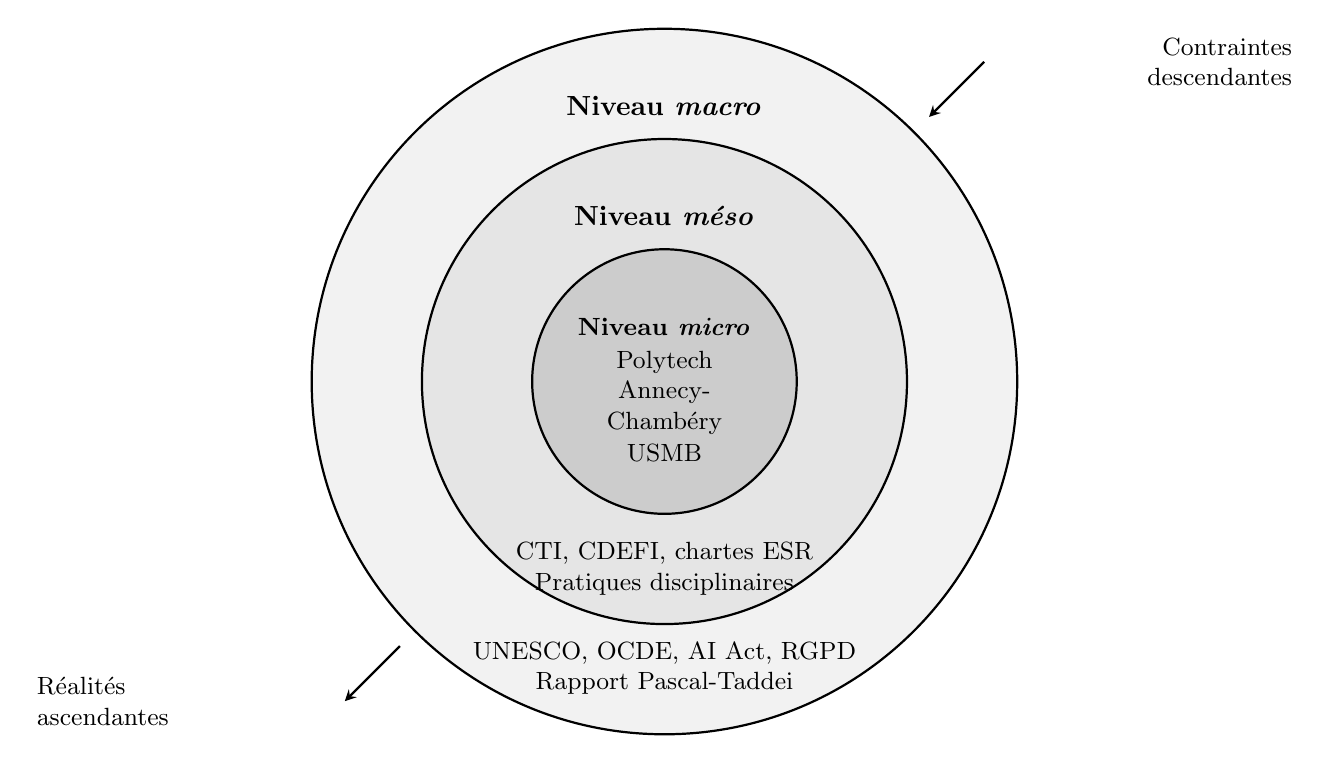
\begin{tikzpicture}[scale=1.4]
  % Cercle extérieur (Macro)
  \draw[thick, fill=black!5] (0,0) circle (3.2cm);
  \node[align=center, font=\normalsize] at (0, 2.5) {\textbf{Niveau \textit{macro}}};
  \node[align=center, font=\small, text width=5.5cm] at (0, -2.6) {UNESCO, OCDE, AI Act, RGPD\\Rapport Pascal-Taddei};

  % Cercle intermédiaire (Méso)
  \draw[thick, fill=black!10] (0,0) circle (2.2cm);
  \node[align=center, font=\normalsize] at (0, 1.5) {\textbf{Niveau \textit{méso}}};
  \node[align=center, font=\small, text width=4.2cm] at (0, -1.7) {CTI, CDEFI, chartes ESR\\Pratiques disciplinaires};

  % Cercle intérieur (Micro)
  \draw[thick, fill=black!20] (0,0) circle (1.2cm);
  \node[align=center, font=\small] at (0, 0.5) {\textbf{Niveau \textit{micro}}};
  \node[align=center, font=\small, text width=2.2cm] at (0, -0.1) {Polytech\\Annecy-Chambéry};
  \node[align=center, font=\small] at (0, -0.65) {USMB};

  % Flèches et annotations
  \draw[->, thick, >=stealth] (2.9, 2.9) -- (2.4, 2.4);
  \node[align=right, font=\small, text width=2.5cm] at (4.8, 2.9) {Contraintes\\descendantes};

  \draw[->, thick, >=stealth] (-2.4, -2.4) -- (-2.9, -2.9);
  \node[align=left, font=\small, text width=2.5cm] at (-4.8, -2.9) {Réalités\\ascendantes};
\end{tikzpicture}
\caption{Architecture en trois cercles concentriques du cadre d'analyse}
\label{fig:cercles_concentriques}
\end{figure}

\subsection{Les sept axes : définitions et justifications}

L'\textbf{Axe 1 — Fondements et état de l'art} constitue le socle conceptuel du projet. Il répond à un besoin de clarification : qu'est-ce que l'IA générative, comment fonctionne-t-elle, quels sont les effets mesurés sur les apprentissages ? Cette dimension technique et scientifique s'avère indispensable pour dépasser les discours d'opinion et fonder les recommandations sur des données probantes. Les méta-analyses récentes~\cite{wang2025meta,deng2025chatgpt} permettent désormais de quantifier les effets pédagogiques avec une rigueur méthodologique satisfaisante.

L'\textbf{Axe 2 — Cadres éthiques et réglementaires} traite de la dimension normative, devenue incontournable avec l'entrée en vigueur de l'AI Act européen~\cite{aiact2024}. L'éducation y est classée secteur à haut risque, ce qui impose des obligations de conformité aux établissements. Cet axe couvre également l'intégrité académique — la définition de la fraude à l'ère de l'IA générative — et l'impact environnemental, dimension émergente mais croissante dans les préoccupations institutionnelles.

L'\textbf{Axe 3 — Impacts pédagogiques} approfondit les effets de l'IA sur les apprentissages : compétences menacées versus compétences à développer, transformation de la relation pédagogique, repensée de l'évaluation. Il s'articule étroitement avec l'Axe 1 dont il constitue le prolongement appliqué, en se concentrant sur les implications pour la conception des enseignements.

L'\textbf{Axe 4 — Pratiques et usages} adopte une perspective empirique : que font réellement les étudiants, les enseignants, les personnels administratifs avec l'IA ? Cet axe descriptif, alimenté par les enquêtes nationales et internationales, permet d'ancrer les recommandations dans la réalité des pratiques plutôt que dans des projections théoriques. Il prépare directement l'enquête de terrain prévue à Polytech.

L'\textbf{Axe 5 — Gouvernance institutionnelle} aborde la dimension organisationnelle : comment structurer le pilotage de l'IA dans un établissement, quel modèle de charte adopter, quelles infrastructures déployer, comment former les personnels ? Cette dimension stratégique, largement documentée par le rapport Pascal-Taddei, conditionne la capacité d'action de l'établissement.

L'\textbf{Axe 6 — IA métier} introduit une distinction essentielle pour une école d'ingénieurs : l'IA n'y est pas seulement un outil pédagogique (apprendre \textit{avec} l'IA) mais aussi un contenu de formation (apprendre \textit{l'IA}). Le machine learning, la vision industrielle, la maintenance prédictive constituent des compétences métiers attendues par les employeurs dans les six filières de Polytech.

L'\textbf{Axe 7 — Spécificités Polytech} ramène l'analyse au niveau micro : état des lieux des maquettes pédagogiques, pratiques existantes, articulation avec l'USMB. Cette contextualisation garantit que les recommandations finales seront opérationnelles et adaptées aux spécificités du terrain.

\subsection{Articulation et cohérence d'ensemble}

Ces sept axes se complètent selon une logique qui va du savoir (A1) au faire (A4, A6), en passant par le devoir (A2) et le pouvoir (A5), pour aboutir à l'être institutionnel spécifique (A7). L'axe 3 joue un rôle charnière entre les fondements théoriques et les pratiques observées. Plusieurs dimensions ont été volontairement écartées : le volet recherche (bien que les recommandations INRIA soient prises en compte) car la mission porte prioritairement sur la formation, et les aspects techniques d'infrastructure détaillés (choix de modèles, déploiement de serveurs) qui sont abordés dans l'Axe 5 de manière synthétique.

Cette structuration en axes thématiques ne reproduit pas directement un cadre existant mais s'en inspire. Le référentiel UNESCO organise les compétences enseignantes en cinq aspects (perspective centrée humain, éthique, fondements, pédagogie, développement professionnel) qui recoupent partiellement nos axes 1, 2 et 3~\cite{unesco2024competences}. Le rapport Pascal-Taddei structure ses recommandations autour de six objectifs qui correspondent globalement à nos axes 5 et 6. La revue systématique de Batista et al. identifie six axes de recherche prioritaires pour l'ESR, confirmant la pertinence des dimensions retenues~\cite{batista2024systematic}. L'originalité de notre approche réside dans l'ajout explicite de l'Axe 6 (IA métier) et de l'Axe 7 (contextualisation locale), absents des cadres génériques mais indispensables pour une école d'ingénieurs. Cette adaptation au contexte particulier de Polytech illustre la démarche de transférabilité critique qui guide l'ensemble du projet : s'appuyer sur les cadres de référence tout en les adaptant aux spécificités du terrain.

Les quatre sections suivantes développent de manière approfondie les axes thématiques majeurs : les fondements techniques et scientifiques (section 3), le cadre éthique et réglementaire (section 4), les pratiques et usages observés (section 5), et la gouvernance institutionnelle (section 6). Les axes 3, 6 et 7, dont le développement dépend de travaux empiriques à venir (enquête de terrain, audit pédagogique), sont abordés de manière transversale dans les recommandations finales.
